\documentclass[aps,prl,twocolumn,groupedaddress]{revtex4-1}

%\documentclass[11pt]{amsart}
%\usepackage{geometry}                % See geometry.pdf to learn the layout options. There are lots.
%\geometry{letterpaper}                   % ... or a4paper or a5paper or ... 
%\usepackage[parfill]{parskip}    % Activate to begin paragraphs with an empty line rather than an indent
\usepackage{graphicx}
\usepackage{amsmath}
%\usepackage{amssymb}
%\usepackage{epstopdf}
%\DeclareGraphicsRule{.tif}{png}{.png}{`convert #1 `dirname #1`/`basename #1 .tif`.png}
\begin{document}

\title{Improving Dark Matter Axion Searches with Active Resonators}
\author{G. Rybka, A. Malagon, L. McBride, K. Patel, Jacob?}
\email[]{grybka@uw.edu}
\affiliation{University of Washington}
\date{}                                           % Activate to display a given date or no date

%runnning list of figures we need in the paper:
%plot of snr vs Q for signal sent in on resonance; with and without delay line
%plot of snr vs Q for a measurement made one peak away from tallest peak
%plot of S_11 with and without delay line
%plot of snr vs Q for the new delay line in the transition region
% all of the above needs to be done with the new couplings as we changed the coupling coefficients
% after shipping the demo delay line back. Ask Lisa what those coupling coefficients are.
% perhaps change the coupling coefficients and see where the sweet spot is for snr improvement?
%

\date{\today}

%copied directly from Gray's original arxiv paper
\begin{abstract}
Axions are a well motivated candidate for dark matter.  The most sensitive experiments searching for dark matter axions rely on the coupling of axions to the electromagnetic resonances of a microwave cavity immersed in a strong magnetic field.  The sensitivity of the experiment is proportional to the $Q$ of the resonance that is coupled to axions.
To date, the resonators used in axion searches have all been passive, with $Q$s limited by power loss in the cavity walls.  I propose the use of active feedback resonators to increase the $Q$ of microwave cavity axion dark matter experiments by several orders of magnitude.
This should allow experiments to significantly increase the rate at which they can test potential axion masses and couplings.
%this is too bold a claim; realistically we can only get to 10^6 before signal power plateaus.
\end{abstract}

\pacs{}

\maketitle

\section{Introduction} 
%copied directly from Gray's original arxiv paper.

The axion is a hypothetical particle that is both a candidate for dark matter and a result of the Peccei-Quinn solution to the strong CP problem~\cite{Peccei,Peccei_2,PhysRevLett.40.223,PhysRevLett.40.279,Preskill1983127,Abbott1983,ipser-sikivie}.
Axions with masses below $10^{-3}$ eV are particularly interesting because they could be produced in sufficient quantities to account for 
%cold
dark matter~\cite{Turner199067}.
For axions in this mass range the coupling between axions and photons
%say two photon coupling?
, despite being exceptionally weak, provides the best chance of directly observing axion dark matter.

The most sensitive dark matter axion searches to date have been of the ``microwave cavity" type.
%somehow the assumption that axions form all of the dark matter halo is lost...
These experiments rely on the conversion of axions from the local dark matter halo into photons in a strong magnetic field.
This conversion is resonantly enhanced when the resonant frequency of the microwave cavity is equal to the frequency of the photons produced from the axion conversion~\cite{PhysRevLett.51.1415}.
%again, the missing information is that axions are non-relativistic, better way to say it is that the energy deposited into the electromagnetic field excites a resonant mode of the cavity. this might be a good time to bring in the energy dispersion.
Operation of these experiments involves slowly tuning the resonant frequency of the microwave cavity to explore different potential axion masses and searching for an excess of power deposited from dark matter axion conversion.
Microwave cavity experiments have been demonstrated to have the sensitivity required to detect optimistically coupled dark matter axions over a small mass range,
%maybe say explicitly from 2-4 microeV
but as of yet, axions have not been detected in a microwave cavity experiment~\cite{PhysRevLett.104.041301}.

The signal power in microwave cavity experiments is proportional to a number of factors, including the local density of dark matter, the strength of the magnetic field, the volume of the cavity, and the resonant 
%loaded
quality factor $Q$ of the resonance being used:
%give equation
\begin{align}
P_{sig} = g_{a\gamma\gamma}^2B_{ext}^2VC\frac{\rho_a}{m_a}\text{max}(Q_{loaded},Q_a)
\end{align}
The primary background is the thermal noise from the physical temperature of the cavity and the electronic noise from the first stage amplifier.  
The figure of merit for a microwave cavity experiment is the instantaneous axion signal to noise ratio (SNR).
%why emphasize instanteneous?
Experiments with a larger SNR can be sensitive to more pessimistic axion photon couplings for a given frequency tuning speed or tune more quickly for a given axion photon coupling sensitivity.

Increasing the cavity $Q$ is one way to increase SNR in a microwave cavity experiment; the speed at which the cavity frequency can be tuned while remaining sensitive to a given axion photon coupling is linearly proportional to $Q$~\cite{Peng2000569}.
The presence of a strong magnetic field precludes the use of high-$Q$ superconducting cavities in these experiments, so the cavities are usually made of or coated with copper.
%add, ``...although R&D is being done with superconducting thing films on the walls...''
Loaded $Q$s of $10^5$ at 1 GHz have been achieved with copper cavities in axion experiments~\cite{Peng2000569}.  Higher frequency cavities typically have smaller $Q$s.
%mention anomalous skin depth limit, or scaling of Q with frequency as f^-2/3?
%The quality factor for a passive resonator depends solely on the frequency, geometry, and material of the resonator.
For a cylindrical copper cavity the Q scales as $Q \propto f^{-2/3}$....skin depth.

I present here a means of artificially increasing the $Q$ of the cavity resonance using active feedback in order to improve sensitivity to dark matter axions and increase the speed at which different axion masses can be tested.

\subsection{Axions, Dark Matter, and Microwave Cavities}

\subsection{Technological Limitations, Overcoming them with Active Resonators}

\section{Schematic}

\begin{figure}
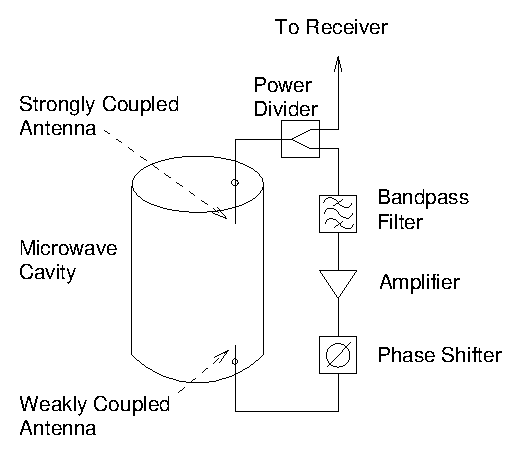
\includegraphics[width=7cm]{figs/experiment_schematic.eps}
\caption{\label{fig:experiment_schematic} Schematic of active feedback resonator for an axion experiment}
\end{figure}

\begin{figure}
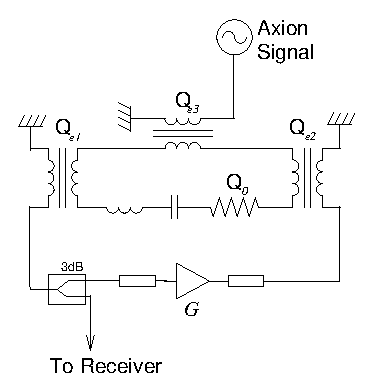
\includegraphics[width=6cm]{figs/equivalent_circuit.eps}
\caption{\label{fig:equiv_circuit} Equivalent circuit to axion photon conversion in microwave cavity with active regeneration}
\end{figure}

\begin{figure}
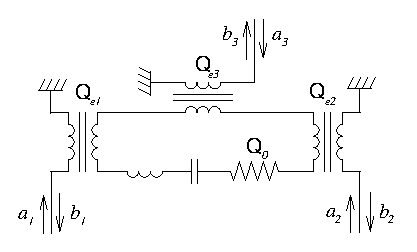
\includegraphics[width=6cm]{figs/amplitude_definitions.eps}
\caption{\label{fig:amplitude_defs} Microwave cavity represented as three port device.}
\end{figure}

The use of active feedback resonators is a well established technique used in regenerative receivers~\cite{armstrong1914wireless}.
It involves connecting positive feedback to a resonator at the appropriate phase and amplification such that the power lost each oscillation to the output and damping effects is nearly completely replaced.  
This has the effect of increasing the $Q$ of the system.
%perhaps say here that it will also amplify the noise of the system. However we show that the SNR improves square-rootishly with multiplier.
A schematic of a microwave cavity axion experiment with active feedback is shown in Fig.~\ref{fig:experiment_schematic}.   Power from axion to photon conversion exits the cavity via a strongly coupled antenna, some of which is sent to a detector.  The remainder of the power is amplified, phase shifted, and then fed back into the cavity via a weakly coupled antenna.  A filter may also be needed to select the desired mode. 


\section{Theory}

\subsection{Derive multiplicative factor to gain}
%We can derive the increase in Q and noise using an equivalent circuit model of the cavity and feedback system.
%We represent the cavity as an RLC circuit, with impedance transformers representing the coupling ports from the cavity to the external system.
%An amplifier with voltage gain $\sqrt{G_a}$ and equivalent noise temperature $T_a$ is placed in the feedback loop along with a phase shifter.
%The closed loop gain of the system, assuming no loss in the phase shifter, is then $\sqrt{G_l} = S_{12}\sqrt{G}$. When 
To calculate the effect of the active feedback, I will use the equivalent circuit to the cavity-amplifier system shown in Fig.~\ref{fig:equiv_circuit}.  The cavity resonant mode is equivalent to an $LRC$ circuit with an unloaded $Q$ of $Q_0$ and the coupled antennas are equivalent to transformers with couplings $Q_{e1}$ and $Q_{e2}~$\cite{Montgomery:1948}.  $G$ is the combined gain of the amplifier and power divider.  There is also a phase shift between the two antennas around the loop, which will be denoted as $\delta$.  The coupling between the electromagnetic resonance in the cavity and dark matter axions is equivalent to a third antenna with coupling $Q_{e3}$.  The passive loaded $Q$ of the resonator is $Q_L=\left(Q_0^{-1}+Q_{e1}^{-1}+Q_{e2}^{-1}+Q_{e3}^{-1}\right)^{-1}$.

I can now treat the cavity as a three port device using amplitudes defined in Fig.~\ref{fig:amplitude_defs} with an $S$ matrix of
\begin{equation}
S_{\mathrm{cavity}}=
\left( \begin{array}{ccc}
		\frac{2Q_L}{Q_{e1}}-1 & \frac{2Q_L}{\sqrt{Q_{e1}Q_{e2}}} & \frac{2Q_L}{\sqrt{Q_{e1}Q_{e3}}}  \\
		\frac{2Q_L}{\sqrt{Q_{e1}Q_{e2}}} & 1-\frac{2Q_L}{Q_{e2}} & \frac{2Q_L}{\sqrt{Q_{e2}Q_{e3}}}  \\
		\frac{2Q_L}{\sqrt{Q_{e1}Q_{e3}}} &  \frac{2Q_L}{\sqrt{Q_{e2}Q_{e3}}} &  1-\frac{2Q_L}{Q_{e3}} \\
		\end{array}\right)
\end{equation}
    assuming the resonant frequency of the cavity has been tuned to the axion frequency.

The output amplitude $b_1$ can be determined with the cavity $S$ matrix
\begin{equation}
\left(\begin{array}{c}
b_1\\
b_2\\
b_3\\
\end{array}\right)
=
S_{\mathrm{cavity}}\left(\begin{array}{c}
a_1\\
a_2\\
a_3\\
\end{array}\right),
\end{equation}
the effect of the amplifier and phase shifter
\begin{equation}
a_2=\sqrt{G}b_1e^{i\delta},
\end{equation}
and $a_1=0$.   I will take $\delta$ to have been chosen to be an integral multiple of $2\pi$.  This gives
\begin{equation}
b_1=\frac{2MQ_L}{\sqrt{Q_{e1}Q_{e3}}} a_3
\end{equation}
where I define $M$ to be the apparent multiplier to the $Q$ of the system
\begin{equation}
M=\left(1-2Q_L\sqrt{\frac{G}{Q_{e1}Q_{e2}}}\right)^{-1}.
\end{equation}
Note that for a passive resonator $M=1$ and that systems with $M<0$ will oscillate regardless of the presence of an axion signal. 
%should that be M>1?
I note that from the signal power derived in Refs.~\cite{Cavity_idea_2,PhysRevLett.80.2043},
\begin{equation}
\frac{|a_3^2|}{Q_{e3}}=g_{a\gamma\gamma}^2VB_0^2\rho_aC\frac{1}{m_a}
\end{equation}
%remove this it doesn't make any sense to discuss amplitude of signal before entering the cavity.
where $V$ is the volume of the microwave cavity, $B_0$ is the magnetic field strength, $\rho_a$ is the density of dark matter axions, $C$ is a mode dependent form factor of order 1, and $m_a$ is the axion mass.  
$g_{a\gamma\gamma}$ is the axion-photon coupling strength, defined as $g_{a\gamma\gamma}=\frac{\alpha g_\gamma}{\pi f_a}$ where $\alpha$ is the fine structure constant, $f_a$ is the axion decay constant and $g_\gamma$ is an order unity model dependent factor.

 The power measured at the output of the system is thus
\begin{equation}
\label{eqn:rawsig}
P_{\mathrm{signal}}=\frac{M^2Q_L^2}{Q_{e1}}g_{a\gamma\gamma}^2VB_0^2\rho_aC\frac{1}{m_a}
\end{equation}

It is important to note that for the isothermal halo model of dark matter axions,  the characteristic width of the axion signal is expected to correspond of a $Q$ of $10^6$ \cite{Cavity_idea}.   Experiments with a bandwidth smaller than the axion signal width sample only a subset of axions.  Thus the conservative estimate for signal power is

\begin{equation}
\label{eqn:sig}
P_{\mathrm{signal}}=\frac{M}{2}\min\left(MQ_L,10^6\right)g_{a\gamma\gamma}^2VB_0^2\rho_aC\frac{1}{m_a},
\end{equation}

though it could be larger in models where the axion dark matter is unusually cold.
%I feel like this way of presenting it is misleading. It's implying we may very well have colder dark matter and could enhance our sensitivity,
%but the reality is that we just don't know, so have to stick to the isothermal model.
The thermal noise from the physical temperature of the cavity and electronic noise of the amplifier are also magnified by the active feedback.

%\section{Theory copied from Ipython Notebook Writeup}
%Referencing the image above, we use the following notation: $N_0$ is the cavity thermal noise power, $N_b$ is the amplifier noise power traveling away from the amplifier, and $N_a$ is the noise power traveling towards the amplifier (referenced to the input of the amplifier). I use lower case to denote the respective voltages, so $n_0$ is the cavity voltage noise, and $|n_0|^2 = N_0$, etc. $\sqrt{G}$ is the voltage gain of the amplifier, with the effective gain of the circuit is given by $\sqrt{G}S_{23}$. The relationship between the input amplitudes $a$ and output amplitudes $b$ is given by the S parameter matrix:
%
%$$
%S = \left(\begin{array}{ccc}
%-1 + 2Q_L/Q_{00} & 2 Q_L/\sqrt{Q_{00}Q_{1}} & 2Q_L/\sqrt{Q_{00} Q_2} \\
%2 Q_L/\sqrt{Q_{00}Q_{1}} & -1 + 2Q_L/Q_{1} & 2Q_L/\sqrt{Q_{1} Q_2} \\
%2 Q_L/\sqrt{Q_{00}Q_{2}} & 2Q_L/\sqrt{Q_{1} Q_2} & -1 + 2Q_L/Q_{2} \\
%\end{array}\right)
%$$
%
%(NOTE: there is a typo in the afr_noise paper by Ishikawa and co. - their $S_{13}$ entry is wrong.)
%
%My understanding of the notation here is that $Q_{00}$ is the unloaded Q of the cavity, $Q_L$ is the loaded Q of the cavity, $Q_1$ and $Q_2$ are quality factors parameterizing the coupling ports, and $Q_0$ is the active Q (unloaded).
%
%TODO: is the S parameter matrix In the language of coupling coefficients, $\beta_1 = \sqrt{\frac{Q_{00}}{Q_1}}$ and $\beta_2 = \sqrt{\frac{Q_{00}}{Q_2}}$.
%
%The relationship between the active Q and the other quality factors is given by:
%
%\begin{align}
%\frac{1}{Q_0} = \frac{1}{Q_L} - 2\sqrt{\frac{G}{Q_1 Q_2}}.
%\end{align}
%
%Physically, the above equation tells us that a loaded cavity quality factor will be further modified by the introduction of gain, which will act as a negative resistance. When 
%
%$$
%\sqrt{G} = \frac{\sqrt{Q_1 Q_2}}{2 Q_L}
%$$
%
%then the active quality factor goes to infinity, and the circuit becomes an oscillator. The equation above is the same as the condition that $S_{23}\sqrt{G} = 1$.
%
%Now that we've established our notation, we want to know what the output power would look like. If we take the output from port 1 ($b_1$) as the voltage we will be listening to, then $b_1$ has the form:
%
%$$
%b_1(t)= S_{21} n_0 + S_{22} n_b + S_{23} \sqrt{G} \big(b_1(t- t_0) + n_a \big)
%$$
%
%Note that we $b_1$ is evaluated at two different times in this equation - once at the current time $t$ but also at $t-t_0$, where $t_0 = L/c$ is the time it takes for a wave at port 1 to traverse the circuit's length $L$.
%
%The time-averaged power we expect then is:
%
%$$
%<|b_1(t)|^2> + |S_{23}|^2 G <|b_1(t-t_0)|^2> - 2 S_{23} \sqrt{G} < b_1^*(t)b_1(t-t_0)> = |S_{21}|^2 N_0 + |S_{22}|^2 N_b + |S_{23}|^2 G N_a.
%$$
%
%where we assumed that there is no correlation between the various noise sources, e.g. $<n_0 n_b> = 0$.
%
%Let us assume a steady state solution such that $<|b(t)|^2> = <|b(t-t_0)|^2>$. The autocorrelation of the two $b_1(t)$ terms is given by (NOTE: ask Gray again about how this was gotten):
%
%$$
%<b_1^*(t)b_1(t-t_0)> = <|b_1(t)|^2> e^{-\omega t_0/Q}
%$$
%
%I drop the subscript $1$ on $b(t)$ for simplicity and denote it by $b_{noise}$. We can rewrite the output power (CHECK: hopefully my transform to frequency space is not sketchy) as
%
%$$
%<|b_{noise}(\omega)|^2> = \frac{|S_{21}|^2 N_0 + |S_{22}|^2 N_b + |S_{23}|^2 G N_a}{1 + |S_{23}|^2 G - 2S_{23}\sqrt{G}e^{-\omega t_0/Q}}.
%$$
%
%Finally, we can parametrize any additional phase shift in the circuit by rewriting $\sqrt{G} \rightarrow \sqrt{G}e^{i\theta}$, so
%
%$$
%<|b_{noise}(\omega)|^2> = \frac{|S_{21}|^2 N_0 + |S_{22}|^2 N_b + |S_{23}|^2 G N_a}{1 + |S_{23}|^2 G - 2S_{23}\sqrt{G}e^{-\omega t_0/Q - i\theta}}.
%$$
%
%Note that we've derived the output noise power in the case of noise signal, but the output power when a signal is injected into the system (ie $a_0 = \sqrt{\beta_0} p$) would only be modified to be:
%
%$$
%<|b_{signal}(\omega)|^2> =\frac{|S_{21}|^2 \beta_0 P}{1 + |S_{23}|^2 G - 2S_{23}\sqrt{G}e^{-\omega t_0/Q - i\theta}}
%$$
%
%so the SNR would be:
%
%$$
%SNR = \frac{<|b_{signal}(\omega)|^2>}{<|b_{noise}(\omega)|^2>} = \frac{|S_{21}|^2 \beta_0 P}{|S_{21}|^2 N_0 + |S_{22}|^2 N_b + |S_{23}|^2 G N_a}
%$$
%
%... this doesn't make any sense. Not sure what I did wrong here.
%
%A different approach would be to recognize that the active Q ($Q_0$) gains by one factor of the multiplier:
%
%$$
%Q_0 = Q_L(1 - \sqrt{G_l})^{-1}
%$$
%
%where $G_l$ is the loop gain ($\sqrt{G_l} = S_{23}\sqrt{G}$).
%
%Then notice that the real gain, (not just through one pass), is given by
%
%$A = n_{cav} + A\sqrt{G_l}$ so $A = n_{cav}/(1-\sqrt{G_l})$.
%
%so if that's the voltage all around gain, then the power gain (all throughout) is $P = N_{cav}/(1-\sqrt{G_l})^2$.
%
%Therefore, for $t_0 = 0$,
%
%$$
%SNR = \frac{P_{in} ( 1- \sqrt{G_l})^2}{(1-\sqrt{G_l})^2 (T_{cav} + G_l T_a)} = \frac{P_{in}}{(T_{cav} + G_l T_a)}
%$$
%
%and for $t_0 = 2.5$ $\mu$seconds,
%
%$$
%SNR = \frac{P_{in} ( 1 + G_l)}{(1-\sqrt{G_l})^2 (T_{cav} + G_l T_a)}
%$$
%
%In any case, for typical experimental parameters, we can plot the noise vs Q for different delay times, which correspond to our measurement configurations with and without the delay line in. See below.

\section{Literature Review}

MENTION ARMSTRONG, MARK JONES
SHOULD WE MENTION DISAGREEMENT BETWEEN ISAKAWA and ITALIAN?

\section{SNR and Bandwidth}
The SNR is given by the ratio of the signal power to the fluctuations in the noise power. We assume that we measure the signal for time $\tau$ with a frequency resolution equal to the width of the axion signal, $B_a$:
\begin{align}
SNR = \frac{P_{sig}}{\delta P_{noise}} = \frac{P_{sig}}{T_{noise}B_a}\sqrt{B_a \tau}
\end{align}

\begin{align}
\text{FIGURE OF MERIT, ACCOUNTING FOR REDUCTION IN BW}
\end{align}

\section{Measurements}

\subsection{Results}

\begin{figure}[htbp]
\centering
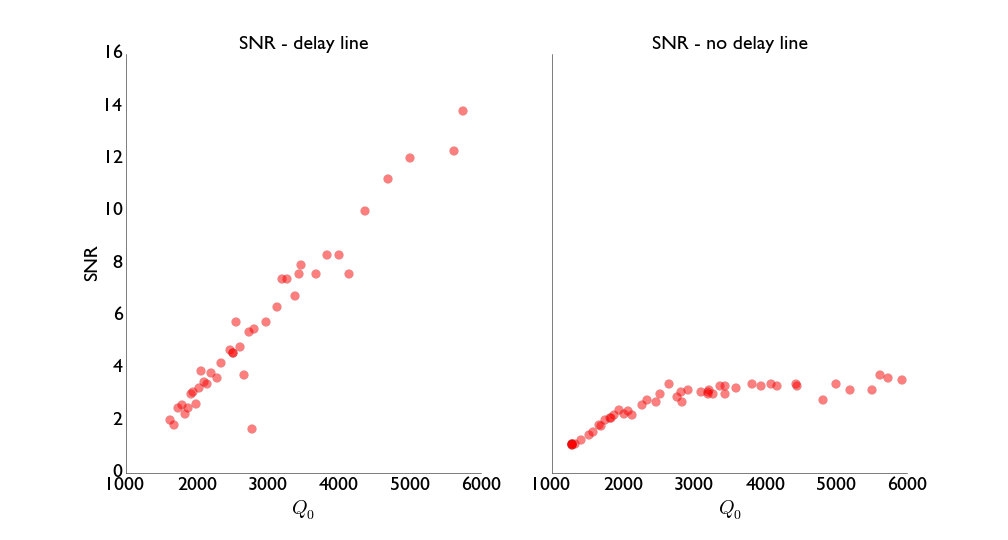
\includegraphics[width=\textwidth]{figs/summary_plots}
\caption{}
\label{fig:summary_plots}
\end{figure}

\subsection{Comparison with Simulation}

\section{Discussion}
Values of $M$ have been reported as high as $10^4$ yielding $Q$s of $7\times10^7$ in active feedback resonators~\cite{:/content/aip/journal/rsi/84/8/10.1063/1.4817537} used for other purposes, but that were operated at frequencies that could be relevant to dark matter axion searches.
This would suggest existing experiments could increase their SNR by several orders of magnitude by implementing active feedback.

The ADMX experiment is within an order of magnitude of the sensitivity necessary to be sensitive to pessimistically coupled axion dark matter.  The addition of active feedback, along with other planned upgrades, should allow it to to be sensitive to pessimistically coupled axion dark matter even in models where axions constitute a very small fraction of the dark matter.  The use of active feedback will also allow future experiments to operate at higher frequencies, where previous microwave cavity experiments have not had the sensitivity necessary to detect axion dark matter with a reasonable scan speed.

This work was supported in part by the U.S. Department of Energy under contract DE-SC0009800.

\section{Wild Speculation}

\bibliography{2014_ouroboros}

\end{document}  
